%********** Chapter 11 **********
\chapter{Conclusions and Future Work}

\section{Conclusions}


\section{Future Work}

Although 3D scanning is relatively an old problem, it is still an important research area, and will continue to be like this because of the continuous improvement in cameras and hardware, which makes it possible to produce results in a faster and more accurate manner.


\subsection{Kinect Development}
Kinect is a very hot supported by Microsoft, this means that Kinect will continue to develop in the future, so it is expected to have better hardware providing better images, it is likely also it will be supported officially on more platforms, also its price is likely to go cheaper making it more and more available.
It's also clear now that Kinect can be used heavily outside the gaming industry, this is why Microsoft launched Kinect for Windows which is a Kinect camera adjusted to work better with Windows.


\begin{figure}[H]
\begin{minipage}[b]{0.5\linewidth}
\centering
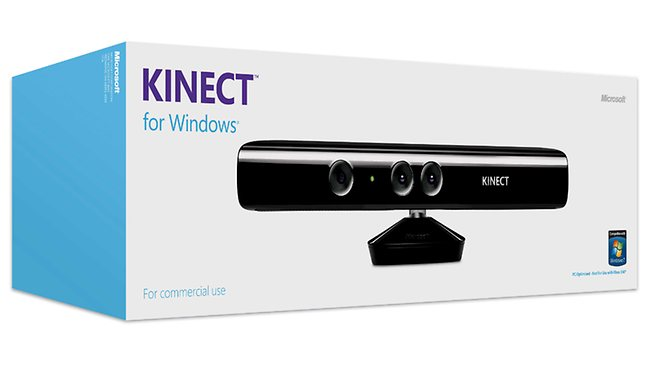
\includegraphics[scale=0.3,keepaspectratio=true]{Conclusions_and_Future/kinect_windows.jpg}
\caption{Kinect for Windows}
\label{fig:kinect_windows}
\end{minipage}
\hspace{0.5cm}
\begin{minipage}[b]{0.5\linewidth}
\centering
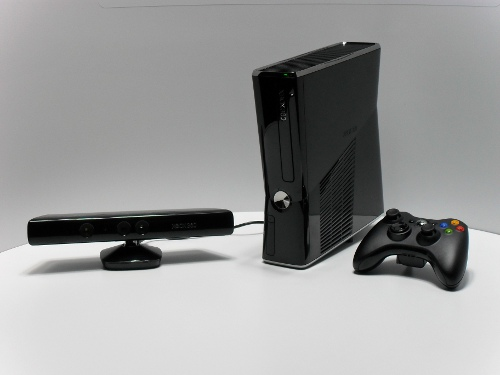
\includegraphics[scale=0.3,keepaspectratio=true]{Conclusions_and_Future/kinect_xbox.jpg}
\caption{Kinect for Xbox}
\label{fig:kinect_xbox}
\end{minipage}
\end{figure}

\subsection{Mobile}

No one can deny how important mobile platforms are in today's world, the mobile market is growing with more tablets and smartphones pushed to the market all over the world, and these mobile devices have considerable computational power and capable hardware.

Smart phones and tablets now have extremely powerfull cameras, we have seen the HTC EVO 3D which is capable of recording and viewing 3D videos, and the new Nokia 808 Pure View which has a 41 mega pixel camera that can take photos of superb quality.

\begin{figure}[H]
\begin{minipage}[b]{0.5\linewidth}
\centering
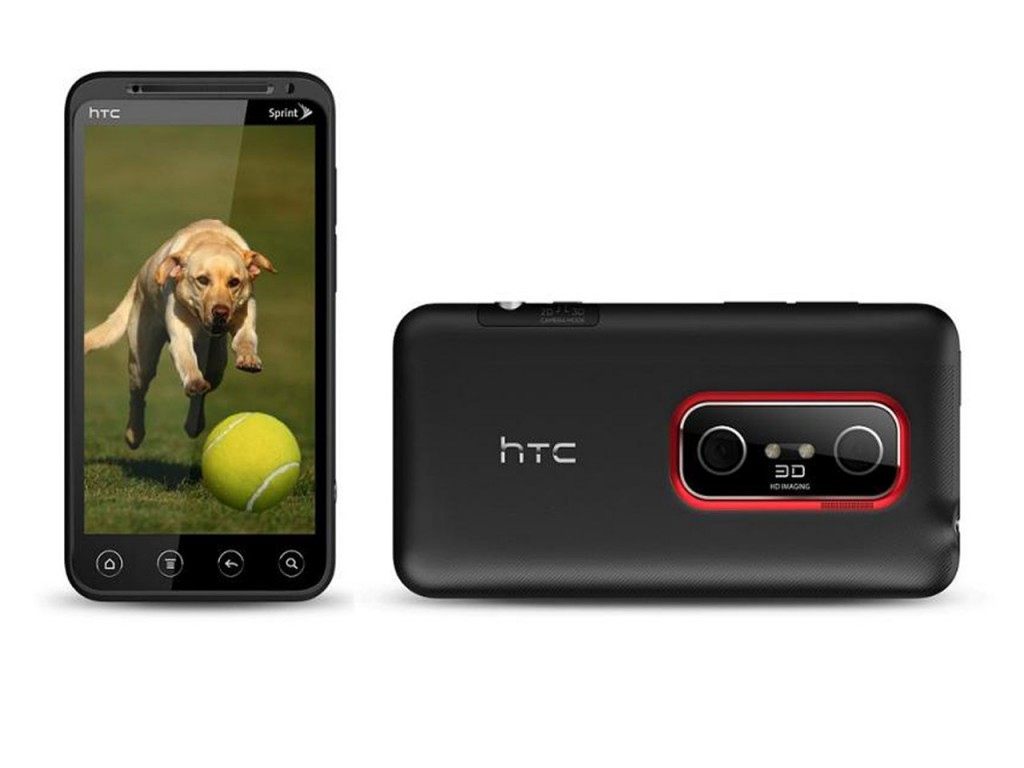
\includegraphics[scale=0.2,keepaspectratio=true]{Conclusions_and_Future/htc_evo.jpg}
\caption{HTC EVO 3D uses two cameras to record 3D videos}
\label{fig:kinect_windows}
\end{minipage}
\hspace{0.5cm}
\begin{minipage}[b]{0.5\linewidth}
\centering
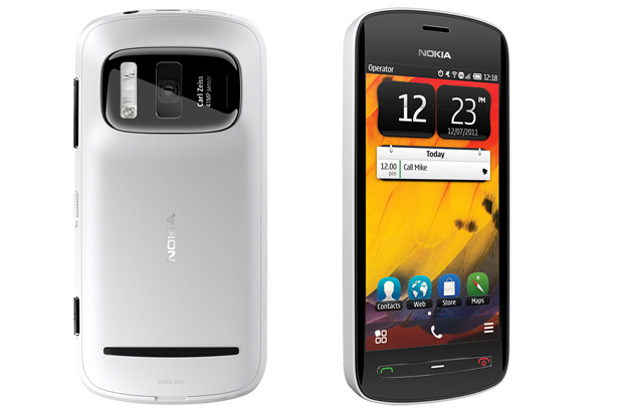
\includegraphics[scale=0.3,keepaspectratio=true]{Conclusions_and_Future/Nokia_808_PureView.jpg}
\caption{Nokia 808 Pure View that can take shots up to 41 mega pixels}
\label{fig:kinect_xbox}
\end{minipage}
\end{figure}

All these new mobile devices show us that at some point in the future we can build SLAM technology inside mobiles, this will open new doors to 3D construction, it will be possible for you to have a 3D model of your vacation beach or hotel room instead of recording a video or taking a photo. The SLAM technology being in the hands of the ordinary user will make it more desirable and demanded which will make researchers and companies work more and more on the technology to prefect it.


\subsection{Walk through}

Our system can be used for advertising for apartments, and it will be a nice feature if the user can actually have a virtual walk through inside the constructed model.

\subsection{Moving Object}

A possible improvement of our system is to add 
